%doc: 2a tramesa revista/cicle_mitja_primaria/Revista 3r-4t 1r trim.doc
\begin{news}
{2} %columnes
{Cinema}
{Al llarg d’aquest curs volem treballar amb els nostres alumnes una petita història del cinema}
{Primaria}
{303} %pagesof

Per això hem escollit una colla de pel·lícules clàssiques que considerem representatives en la història del cinema i a la vegada suposem que  seran motivadores, tot intentant educar el gust per veure pel·lícules de qualitat i evitant el mal costum de mirar sense pensar, sense gaudir de  les imatges i, potser, el més important, aprenent a ser crítics amb el bast món de la imatge.

\subsection*{Primera pel·lícula KING KONG 1933}

\noindent\fbox{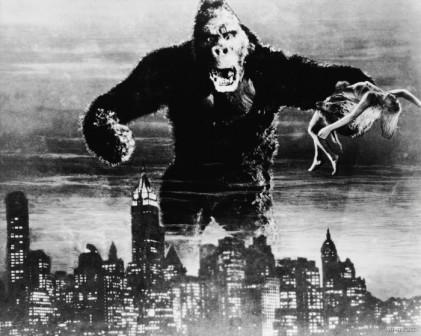
\includegraphics[width=8cm,keepaspectratio]{primaria/img/imgKingKong4.jpg}}

Dibuix de Roger Ibars

\subsubsection*{Mario Rodenas}

A la nostra classe i a la dels nostres companys de quart fem tardes de cinema.

Treballem el Llenguatge audiovisual i el cinema. Fa uns dies vam veure la peli del KING KONG per veure com es feien les pel·lícules abans en el temps antic i també per treballar els plans.

La pel·lícula començava i acabava a New York, i en King Kong moria per salvar la noia.



\noindent\fbox{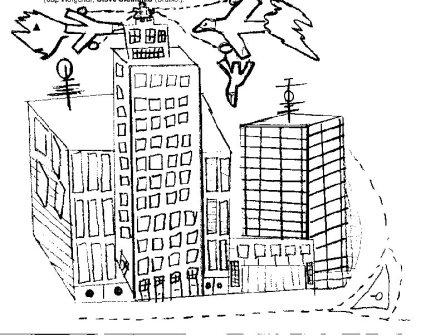
\includegraphics[width=8cm,keepaspectratio]{primaria/img/img099.jpg}}

\subsubsection*{Pol Hernández}
Fa pocs dies vam veure la pel·lícula del King Kong. 
King Kong és un goril·la molt alt i gran.
Em va agradar perquè a mi m’agraden els vaixells i els dinosaures. El que em va agradar més va ser quan estava lluitant amb el Tiranosaurus  Rex.
Després van començar a tirar-li bombes i es va desmaiar i el van portar a New York.



\subsection*{Segona pel·lícula EL HALCÓN Y LA FLECHA 1950}
\noindent\fbox{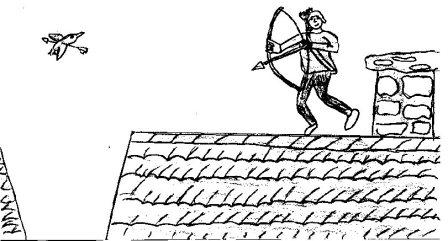
\includegraphics[width=8cm,keepaspectratio]{primaria/img/img097.jpg}}
Dibuix de Santi Gómez

\subsubsection*{
Guim Ordaz
}

En aquesta pel·lícula el protagonista és el Dardo, un noi del poble. Tenen segrestat el seu fill al castell. Els seus amics i ell el volen rescatar i es disfressen de joglars per poder-hi entrar. Després de molt lluitar rescaten el fill i el Dardo comença a saltar d’alegria.
Aquesta pel·lícula m’ha agradat perquè és d’acció i perquè m’agraden els arquers.


\noindent\fbox{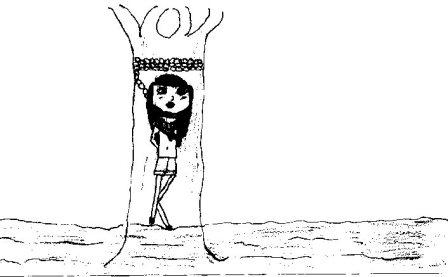
\includegraphics[width=8cm,keepaspectratio]{primaria/img/img098.jpg} 
}
Dibuix de Irene Cuadra

\subsubsection*
{Anna Robles}
Dardo viu a les muntanyes amb el seu fill, són enemics del Duc Urbis conegut amb el nom de “Halcón” que li ha robat la seva dona. Els soldats del Duc fereixen el Dardo  i el seu fill Rudi es deixa capturar per salvar-lo.
Per venjar-se, en Dardo segresta la neboda del Duc que es  diu Ann ...



%Roger Ibars....img 099
%Irene Cuadra...img098
%Santi Gómez...img097

\end{news}
